% 
% Licensed to the Apache Software Foundation (ASF) under one
% or more contributor license agreements.  See the NOTICE file
% distributed with this work for additional information
% regarding copyright ownership.  The ASF licenses this file
% to you under the Apache License, Version 2.0 (the
% "License"); you may not use this file except in compliance
% with the License.  You may obtain a copy of the License at
% 
%   http://www.apache.org/licenses/LICENSE-2.0
% 
% Unless required by applicable law or agreed to in writing,
% software distributed under the License is distributed on an
% "AS IS" BASIS, WITHOUT WARRANTIES OR CONDITIONS OF ANY
% KIND, either express or implied.  See the License for the
% specific language governing permissions and limitations
% under the License.
% 


This chapter provides architectural and implementation details for the DUCC
Resource Manager, referred to as the ``RM''.
\section{Introduction}

The DUCC Resource Manager is responsible for apportioning cluster resources to the
collection of ``work'' to be run by users.  Work is classified into several categories.  As
exposed in the public interface, these categories are:

\begin{description}
  \item[Fair-Share Job] This is a UIMA/AS job, consisting of a minimum of two processes and 
    a potential maximum of as many processes as physically fit on a cluster.  The work
    executed by the processes is parallel, enabling the RM to expand or contract
    the job by allocating or deallocating processes as needed to balance the load.

    Load is balanced using a weighted fair-share policy in which all users are apportioned an
    equitable amount of the cluster resources, where ``cluster resources'' refers only to real
    memory on the cluster nodes.

  \item[Service Instance] This is any arbitrary process that DUCC manages as a ``service''.
    Services are registered with the Service Manager and may be comprised of multiple physical
    processes.  (See the DuccBook for details of DUCC Service Management.)  The RM schedules these
    processes as singletons, using a non-preemptive policy (FIXED\_SHARE or RESERVE).

  \item[Arbitrary Process or ``Managed Reservation''] These are singleton processes of any type, scheduled
    using a FIXED\_SHARE policy.

  \item[Fixed-Share Job] This is a UIMA-AS job scheduled with a non-preemptable, i.e. FIXED\_SHARE
    policy.

  \item[Reservation] This is a request for a dedicated full machine.
\end{description}

The RM is a memory scheduler only.  The use case which justifies DUCC is UIMA-AS jobs, each of
which consists a variable number of parallel processes, each of which requires large amounts of memory, usually
on the order of 16GB or more.  Memory requirements completely overwhelm other resource
requirements, so that jobs scheduled by their declared memory sizes usually get sufficient
other resource such as CPU. 

\section{Vocabulary}
    In order to understand RM it is necessary to understand some of the language used in RM.

    \begin{description}
    \item[quantum] This is the smallest memory size of an allocation, defined in multiples of GB.  It
      is defined globally in {\em ducc.properties} and may be overridden in {\em ducc.classes} for
      top-level nodepools.  See the DuccBook for more details.
      
      Note that although DUCC defines a quantum, most of the RM does not
      use quantum at all; instead it generalizes quantum into {\em qshare}, {\em nshare},
      and {\em order} as defined below.  When a schedule is returned to the Orchestrator, the
      allocations, in terms of quanta, are translated back to memory allocations using this
      configured {\em quantum}.
      
    \item[qshare] This is an abstract memory allocation representing exactly one {\em quantum}.  Memory
      allocations are made in terms of some multiple of {\em qshares}.

    \item[nshare] This is an allocation which consists of one or more co-located {\em qshares}.  When 
      exposed outside of RM this is usually thought of as a ``process''.  It means, literally,
      ``n qshares''.  
      
        Be careful, an {\em nshare} is NOT a process, it is an allocation that can be put to
        any use or to no use if desired.  The RM does not care what an {\em nshare} is used for.

      \item[order] This is a number which refers to the number of {\em qshares} associated with some
        entity such as a machine, a job, a process, an {\em nshare}.  An ``order 3'' machine is a
        machine whose memory can be counted as ``three qshares''.  An ``order 3'' job is a job whose
        processes must be allocated as ``three qshares'' each, or one ``order three'' nshare.

        All {\em qshares} are of order 1, but we don't know how much that is without knowing
        the {\em quantum}.  

        {\em Order} is an abstraction of the {\em quantum}.  Knowing the {\em order}
        of any entity does not tell one how large that entity is.  It does tell one
        how big that entity is in relation to other entities.

        Note that {\em order} is NOT an allocation; it is not a {\em qshare} or an {\em nshare}.
        It is a number which describes the size of things, without saying how big that size
        is or what that thing is.

        Order is used throughout the RM to index arrays and is one of the most fundamental
        concepts in the RM architecture.
      \end{description}
      
\section{Architectural Overview}
    Throughout this section, please refer to the diagram in \hyperref[fig:rm-structure]{Figure ~\ref{fig:rm-structure}}.
    The diagram shows the normal flow through the scheduler, from the time and Orchestrator
    publication arrives to the time the RM publishes its schedule.

\subsection{The Onion}
    At the highest level of abstraction, the RM consists of three layers as seen in the 
    \hyperref[fig:rm-structure]{Figure ~\ref{fig:rm-structure}} below.  It can be thought of as a three-layer onion:
    \begin{description}
    \item[JobManagerConverter] This is the outer layer.  This layer communicates with the
      ``outside'' world: the DUCC Orchestrator and DUCC agents.  It is conceived of as in
      ``impedance matcher'' that converts incoming messages to the RM's internal structures, and
      converts the RM's internal structures into structures recognized by the outside world (the
      DUCC Orchestrator). It is possible to replace this layer without affecting the RM proper; for
      example, to create an isolated simulator for RM development.
    \item[Scheduler] This is the middle layer.  It communicates on one hand with the {\em JobManagerConverter}
      to receive and send data outside of RM and on the other, with the inner layer, the {\em NodepoolScheduler}.
     \item[NodepoolSchedler] This is the inner layer and is the ``scheduler proper''.  Its input is
       a set of allocation requests and its output is a set of node assignments for each request.  These are
       passed up through the {\em Scheduler} and again up to the {\em JobManagerConverter} for publication.
    \end{description}
    
\subsection{Nodes, Machines,  and Node Management}
    The resources scheduled against are nodes.  On each physical node is a DUCC Agent which
    publishes a regular ``heartbeat''.  The ``heartbeat'' contains data describing the
    characteristics of the node used for scheduling: the memory size, the node name, the 
    node IP.  

    If a node fails, its ``heartbeat'' stops arriving.  After some number of missed
    heartbeats, the RM considers the node to be unusable; it will stop scheduling work
    to that node and attempt to evict existing work from the node.  Work that can
    be rescheduled (fair-share jobs and services) get rescheduled on working nodes.

    It is possible to remove a node from scheduling without the node failing using the
    {\em vary\_off} utility.  This causes the RM to stop scheduling work to the 
    specified node, and it causes fair-share work to be evicted and rescheduled elsewhere.

    The RM component responsible for managing nodes is {\em NodePool.java}.  As each
    node heartbeat arrives, the {\em NodePool} is notified and, if it is the first
    such notification, creates an object RM calls the {\em Machine} to represent the
    remote resource.

    The RM implements multiple nodepools in a nested or tree structure.  There is one NodePool
    object for each configured nodepool.  The NodePools are structured in a self-organizing
    tree (that is, none of the Java collection classes are used to organize multiple nodepools).
    Most of the methods inside the NodePool module are recursive, aware of their parent
    NodePools and child NodePools.

\subsection{Jobs}
    The RM is mostly unaware of the purpose for which allocations are made.  It uses a
    single structure, the {\em RmJob} to represent all work.  There are a small number
    of minor switches in the code in deference to specific types of work (UIMA-AS jobs
    vs reservations, for example) but these are not sufficient to justify a more elaborate
    object structure.

\subsection{Shares and share-order}
    All RM allocations are in terms of {\em shares}. A share represents some portion
    of the real memory on a node.  The smallest {\em share} than can be allocated is
    called a {\em quantum share}.  The size of the {\em share quantum} is declared
    in {\em ducc.properties} and can be overridden for {\em top-level nodepools} in
    {\em ducc.classes} (see the DuccBook for the details of quantum configuration).

    In the RM, a single quantum share is called a {\em Qshare}.  Multiple co-located {\em qshares}
    may be allocated for any given request.  A multi-qshare allocation is called an {\em nshare}. A
    {\em nshare} always corresponds to 
    \begin{itemize}
      \item A single process of a FAIR\_SHARE job,
      \item A single process of a FIXED\_SHARE job,
      \item A single service instance process,
      \item A single AP (or ``managed reservation'',
      \item A single unchanged reservation.
    \end{itemize}

    Thus a job may be allocated multiple {\em nshares}.  {\em Nshares} are usually exposed outside
    of RM under the term {\em process}.  (There is a difference: an {\em nshare} refers to an
    abstract allocation; a {\em process} refers to some physical process running on a node.  RM only
    needs to deal in abstractions.)
    
    The term {\em share-order} is used to refer to the number of {\em qshares} associated with
    an entity.  Entities with associated {\em share-order} include
    \begin{itemize}
      \item Jobs.  The {\em share-order} of a job is the number of {\em qshares} required
        to make a single {\em nshare}.  It is a translation of the job's declared memory
        requirements into the number of share quanta required per process.
      \item Nodes (Machines).  The {\em share-order} of a machine is the number of
        {\em qshares} that can be allocated on that machine.  It is a translation of the
        machine's real memory into the number of share quanta that can be allocated to the machine.
      \item Shares.  The order of a {\em share} is the number of {\em qshares} represented
        by the {\em Share} object.  Note this implies that a {\em Share} object always
        represents a single {\em Nshare}.
    \end{itemize}
    
    All of the important algorithms in the RM involve managing incoming work and
    resources by their ``order''.

    A Job's memory specification are converted to {\em share-order} thus:
\begin{verbatim}
    share_order = job_declared_memory / share_quantum
    if ( job_declared_memory % share_quantum ) > 0
        share_order + share_order + 1
\end{verbatim}
    Note that a job's share order is always rounded UP.    
    
    A Machine's announced memory is converted to {\em share-order} thus:
\begin{verbatim}
    share_order = (int) (allocatable_mem / share_quantum;
\end{verbatim}
    Note that a machine's share order is always rounded DOWN.

\subsection{Users}
    Every job that arrives has an associated user.  The RM maintains a map of all users and
    maintains a two-way map of jobs-to-users.  Note that every job has exactly one {\em user} 
    but that every user may have an arbitrary number of {\em jobs}.  Thus, a user may
    be associated with work of different {\em order}s and running in different {\em classes}
    under differing policies.  The structure defined in {\em User.java} maintains all
    necessary records as used by the scheduler.

\subsection{RM Structure Schematic}
    \begin{figure}[H]
      \centering
      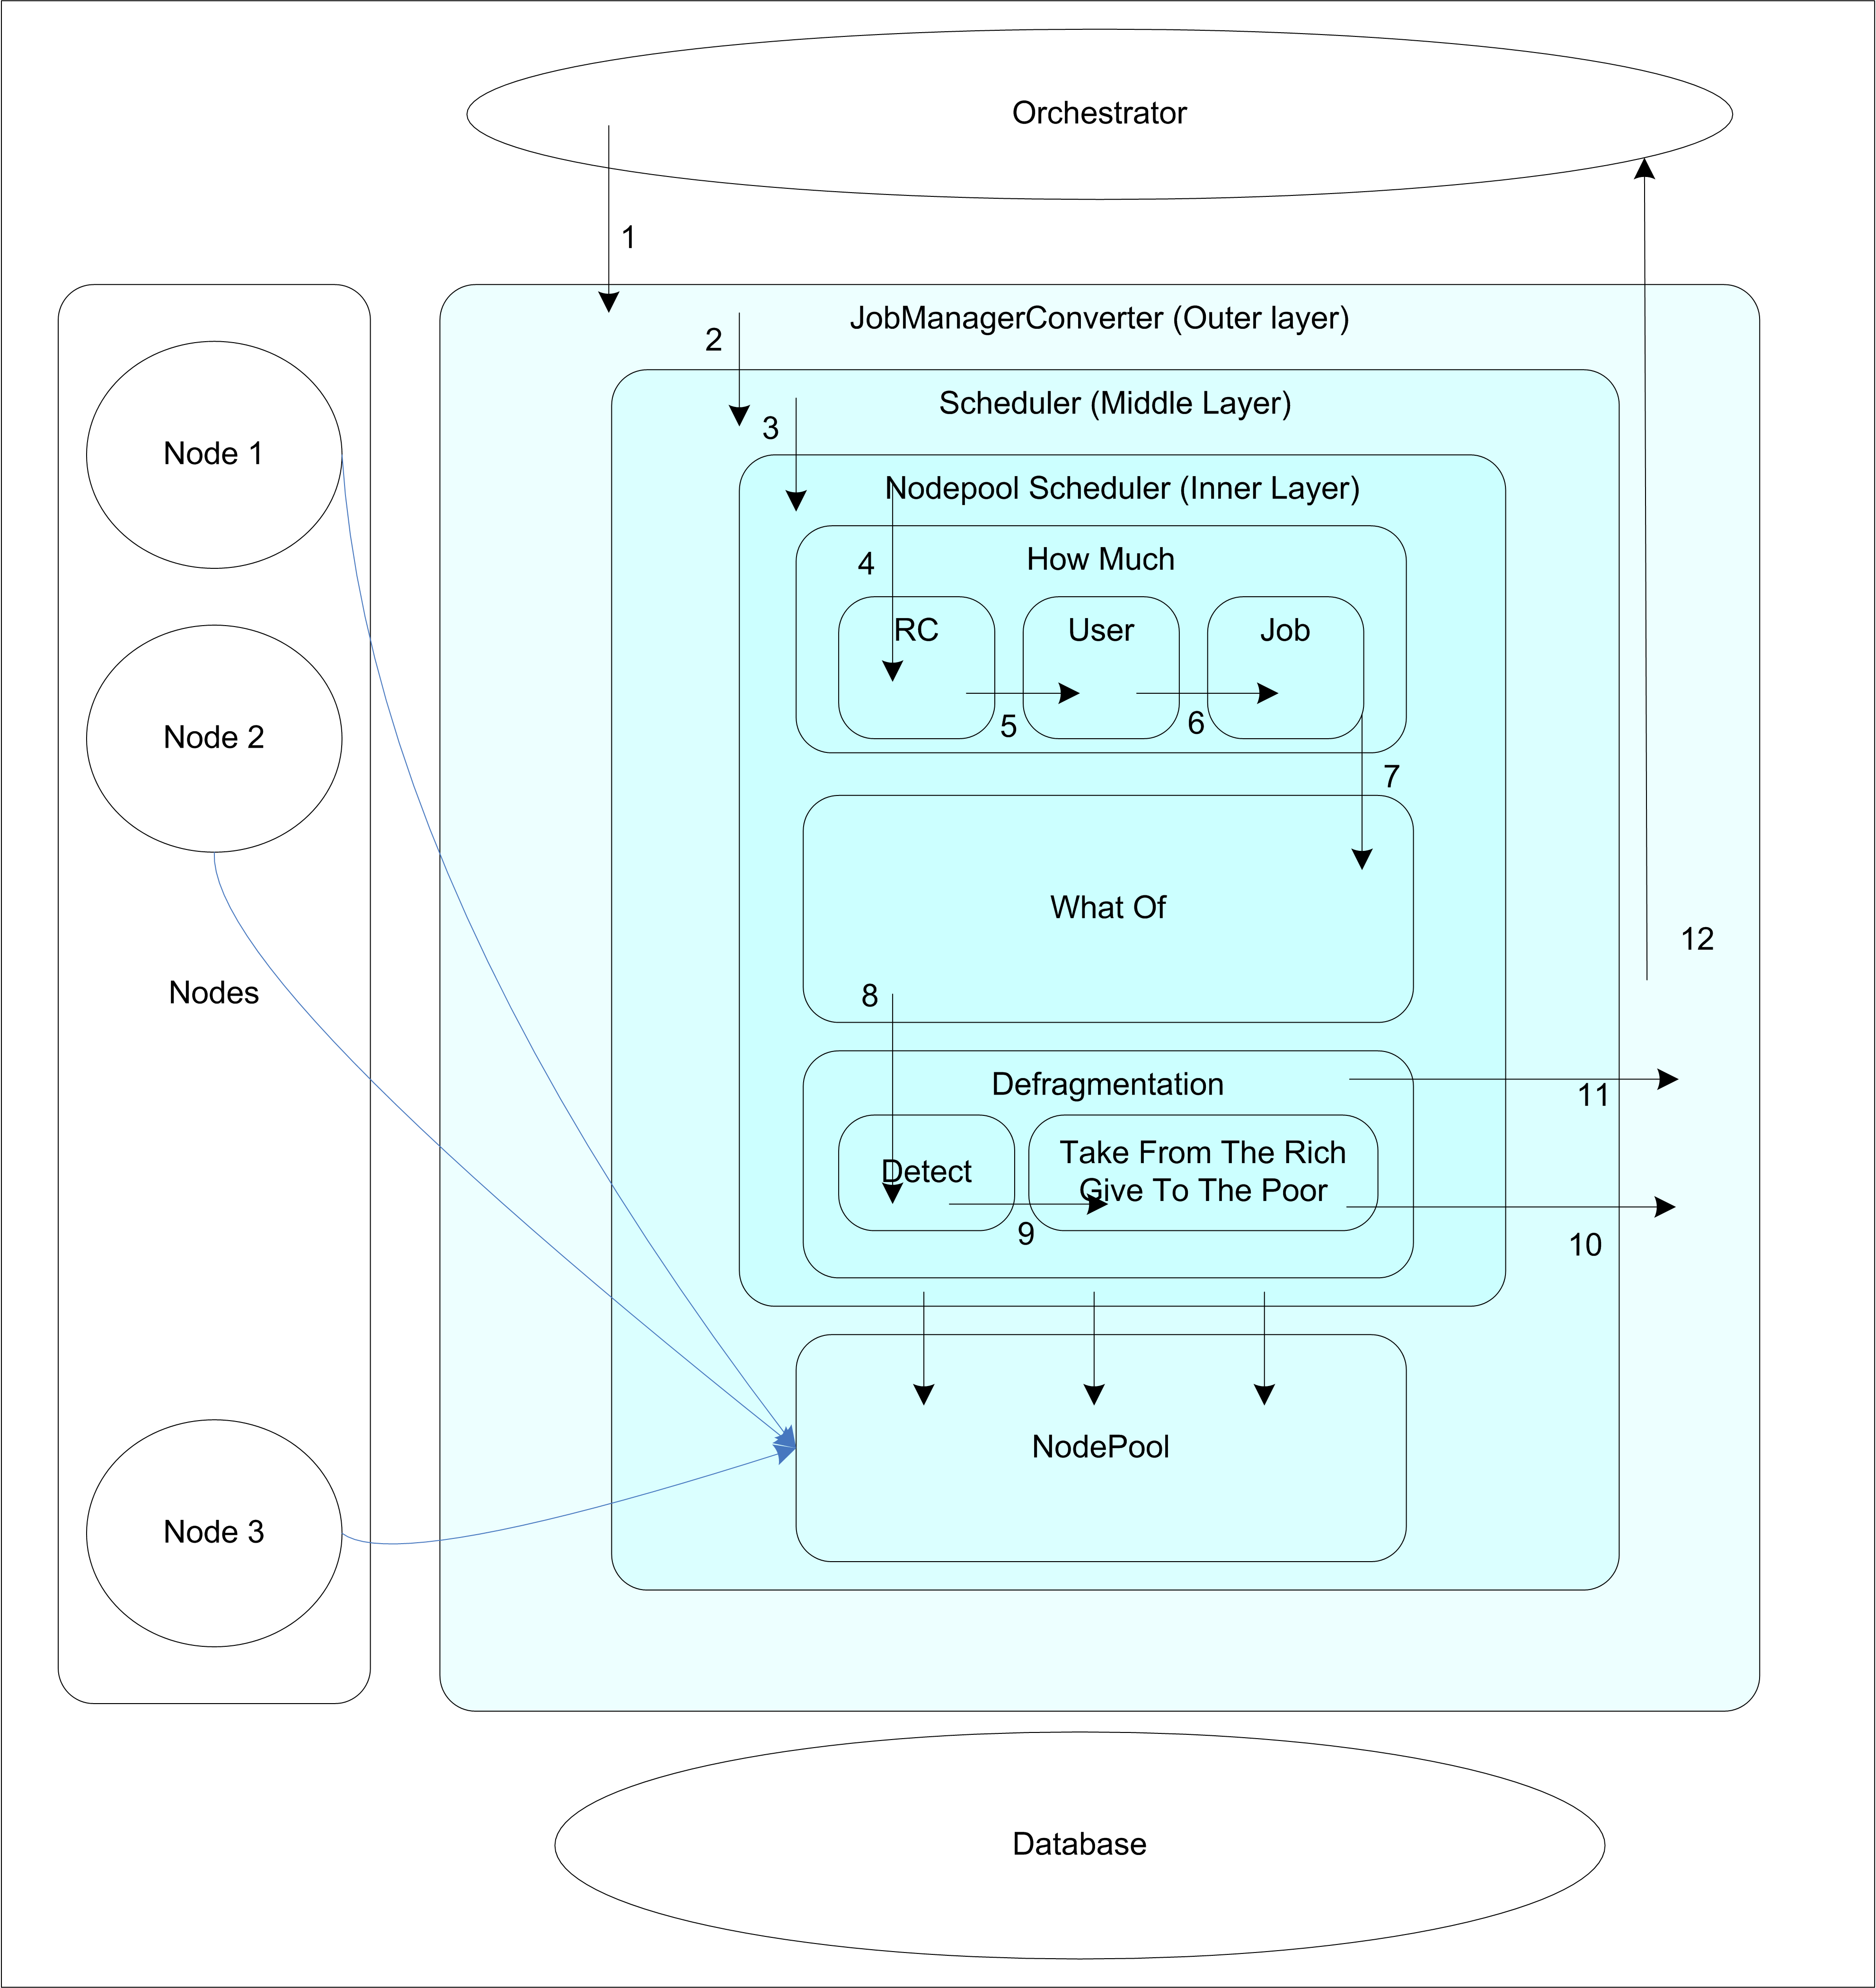
\includegraphics[width=5.5in]{images/ducc-internals/rm-structure.png}
      \caption{RM Structure}
      \label{fig:rm-structure}
    \end{figure}

\section{Outer Layer: JobManagerConverter}

    The {\em JobManagerConverter} is the outermost layer of the RM.  It is intended as a
    buffer or ``impedance matcher'' to protect the RM from the ``outside world''.  It is
    also intended to be replaceable as needed. It communicates with the middle layer through
    an interface.   Any entity that (correctly) uses this interface may act as the outer layer.

    This section describes the most important
    functions of the {\em JobManagerConverter} in detail.  We refer to this as the 
    JMC for brevity.

    The primary function of the JMC is to receive incoming work in the form of Orchestrator
    publications and convert them into a set of discrete scheduling events to be passed to the inner
    layers of the RM.

\subsection{Incoming Work}
    Key methods involved in receiving work and passing it to the next layer are described here.

    \paragraph{eventArrives()} receives the {\em DuccWorkMap} from the Orchestrator.  

     If the RM is not yet initialized the map is ignored.

     If the RM has been recently reconfigured, all structures in JMC are cleared and 
     state set as if this is the first publication.

     If this is the first publication, we pass the map to the method {\em recoverFromOrchestrator}
     to initialize essential structures for work that has {\em ALREADY} been scheduled and is
     running in other parts of the system.  This step is needed for these cases:
     \begin{itemize}
       \item DUCC is being started ``warm''.  In this case the Orchestrator map may include
         Reservations, which are permanently scheduled, and must be recovered. 
       \item The RM may have been stopped (or crashed) and is being restarted.  In this case
         work of all sorts that was already scheduling must be recovered.
       \item The RM may have been dynamically reconfigured.  Dynamic reconfiguration requires
         that all internal structures be reset.  This is the equivalent to stopping and then
         restarting the RM.  Work must be recovered.
     \end{itemize}
     
     The incoming map is now saved for the map-difference code.  If this is the first publication,
     RM simply returns.

     All subsequent Orchestrator publications are compared with the previous map and
     all differences are converted to scheduling events. 

     There are three types of events:
     \begin{description}
       \item[New work] If the work has never been seen before, it is passed to the method
         {\em jobArrives} for conversion into the RM internal structure {\em RmJob}.  The new
         work is passed to the middle layer {\em Scheduler} via {\em signalNewWork()}.
       \item[Completed Work] If the work is marked {\em completed} by the Orchestrator it is
         removed from the local map and the {\em Scheduler} is signalled via {\em signalCompletion()}.
       \item[Existing Work] The associated {\em process map} for each DuccWork object is differenced against the
         previous map to identify processes which may have
         completed or otherwise changed state.  The {\em RmJob} is fetched from {\em Scheduler} and
         the state of its shares or the job itself is updated.  If a process is completed,
         the {\em Scheduler} is signalled via {\em signalCompletion()}, overloaded on share instead of job.  If
         at least one process has reached the {\em Running} state the {\em RmJob} is notified so
         the {\em expand-by-doubling} policy can be enacted.
     \end{description}

     Once the incoming events are processed the middle layer is signaled by invoking the method
     {\em schedule()}.

\subsection{Outgoing Events}
     A schedule is returned from {\em Scheduler} in the form of a {\em JobManagerUpdate} object.  This
     object must be translated into an outgoing publication of the form expected by the Orchestrator.  The
     {\em JobManagerUpdate} is passed to the {\em JobManagerConvert.createState()} method for conversion.

     The final publication is returned in the form of a {\em RmStateDuccEvent} which is then passed to the
     Camel framework for publication.

\section{Middle Layer: Scheduler}

    The ``middle layer'' is implemented in {\em Scheduler.java}.  This entity must conform to the
    interface {\em ISchedulerMain} to maintain the layered ``onion'' architecture.  The ``outer layer''
    does all its interactions with the scheduler proper through this interface.

    The middle layer is relatively straightforward.  It is the middle-man between the {\em JobManagerConverter}
    and scheduler proper, responsible for initialization, global bookkeeping, and dispatching of events
    to the correct objects.  We'll simply list the important functions
    and how to find them:

    \begin{description}
      \item[Initialization] {\em Scheduler.init()} is called from the DUCC infrastructure for RM,
        {\em ResourceManagerComponent}.  RM configuration from {\em ducc.properties} is loaded, the
        class configuration from {\em ducc.classes} is loaded, the RM configuration is announced to the
        log, the database of dynamic RM data is cleared, and the ``initialized'' flag is set to ``true''.
      \item[Class configuration] This ({\em initClasses()}) is invoked out of {\em init()}.  The class configuration is loaded
        into the common {\em NodeConfiguration} object and a set of {\em ResourceClass} objects is
        created.  The {\em NodePool} objects are instantiated.
      \item[Re-configuration] This is implemented in the {\em reconfigure()} method.  Most internal structures
        are cleared and released and {\em init()} invoked as described above.
      \item[Node Publications] All node publications are passed to the method {\em nodeArrives()}. This
        method does a bit of bookkeeping, works out the {\em order} of the node, records the {\em node heartbeat},
        and passes the node to its NodePool for future scheduling.
      \item[Run Scheduler] The {\em schedule()} method is invoked from the outer layer as described
        in the previous section.  This method drains incoming events, ``recovers'' any
        previously-scheduled work, updates state to reflect processes which have exited, and enters
        new jobs and users into the system.  It then invokes the ``inner layer'', the {\em
          NodePoolScheduler} on each top-level nodepool.  This results in creation of the new
        schedule which is passed back to the outer-layer for publication by means of the {\em
          dispatch()} method.
      \item[Dispatch] This method ({\em dispatch()}) records the current schedule in the log
        and converts the schedule into a form usable by the {\em JobManagerConverter} for publication. The
        object created here, {\em JobManagerUpdate} is passed up and published.
      \item[CLI] All CLI methods are handled here, passed in from the outer layer from {\em ResourceManagerComponent}.
        
    \end{description}

\section{Inner Layer: NodepoolScheduler and NodePool}
   The {\em NodePoolScheduler} and it's helper {\em NodePool} comprise the ``scheduler proper''.  They are
   both relatively complex.  This section discusses their architecture and the general flow of data
   through them.  Readers would be advised to have code listings handy if the goal is to fully understand
   the DUCC Scheduler.

   The {\em NodepoolScheduler} is the ``main'' scheduler.  An analogy would be that it is the ``frontal cortex''
   of the brain, doing most of the abstract reasoning required to form a schedule.

   The {\em NodePool} is a helper class, responsible for managing physical layout of processes ({\em ``nshares''})
   over physical nodes ({\em Machines}).  It can be thought of as the ``cerebellum'', controlling the ``arms and legs''
   of the schedule.

    The scheduling rule {\em ``priority''} is implemented by executing the {\em How Much} and {\em
      What Of} phases once for each priority, starting with the ``best'' priority, down to the
    ``worst'' priority.  At each stage the scheduler attempts to give away all of its
    resources. Each subsequent cycle through this loop will generally have fewer resources to
    allocate until either all work is scheduled, or all resources are exhausted, whichever comes
    first.

    After the first two phases are complete in all passes, all fair-share jobs are iterated and any job whose
    physical allocation exceeds the number of resources counted in the ``How Much'' phase has its surplus
    processes preempted.  (These preempted resources are NOT added back to the resource pools until the Orchestrator
    confirms they have exited; hence they aren't accounted for in the ``what of'' phase AT THIS POINT. They
    will be used once they are known to be free.)

    Finally, the {\em defragmentation} phase is executed.

\subsection{NodepoolScheduler}

    We will use a ``divide and conquer'' approach to describe the {\em NodpoolScheduler}.  This component consist of
    three primary parts:
    \begin{description}
      \item[How Much.]  This phase performs the FAIR\_SHARE calculations as well as works out the
        allotments for FIXED\_SHARE and RESERVE requests.  It assumes an ``ideal'' configuration of
        nodes with no conflicts and no fragmentation.  There is one {\em How Much} method for
        each of the three scheduling policies ({\em howMuchFairShare(), howMuchFixed(),} and
        {\em howMuchReserve()}.
          

      \item[What Of.] This phase works closely with the {\em NodePool} to try to find available
        space for the abstract allocations produced by the ``How Much'' phase.  It is responsible for initiating
        preemptions but it never preempts a job below the counts from the ``How Much'' phase.  It preserves
        a stable layout by never preempting work that is already allocated unless that work is exceeds
        some user's fair share as determined by the ``counts'' from ``How Much''.
        
        Note that because it is constrained by the existing layout it may not always succeed
        laying out all work.  If this occurs we must perform ``Defragmentation''.

        The three relevant methods are {\em whatOfFairShare(), whatOfFixed(),} and {\em whatOfReserve()}.

      \item[Defragmentation] After ``What Of'', a pass is made to insure that every job is allocated
        its fair share.  If not, defragmentation is performed to insure that at least ``some minimum'' 
        number of processes is allocated for every job.  This may involve preemptions
        of job processes even for user whose allocations are at or below their fair share.
    \end{description}


    We now describe these three actions in detail.

\subsubsection{How Much}

    For non-preemptive work this is straightforward: the work is assigned whatever is asked for UP TO
    the configured user allotment (see the DuccBook for details of allotment).  Non-preemptive work 
    belonging to users who are at or over their allotment is deferred and not passed to further scheduling stages.

    The FAIR\_SHARE algorithm is performed on each of three {\em entities}: The ResourceClass, the User, and
    the RmJob.  Throughout the rest of the discussion the term {\em entity} is used to refer to any
    of these when the specific type of object is not relevant.  (Each of these entities implement the
    generalized {\em IEntity} interface.).

    \begin{description}
      \item[ResourceClass] Every {\em ResourceClass} is asked to provide a summary of how many {\em nshares}
        of each size it could use, assuming unbounded resources, (but constrained by RM rules such
        as initialization cap and expand-by-doubling).  They produce an
        array, indexed by {\em share order} of the number of processes of each order they want allocated.

        To produce this array, the {\em ResourceClass} iterates all jobs ({\em RmJob} structures) assigned to the class and ask 
        the same question of the RmJobs:, ``in an unbounded world what is the maximum number of processes you require''.  The
        method responding, {\em RmJob.getJobCaps()} examines the number of work items not-completed, the number
        of threads per process, and their {\em process\_deployments\_max} to produce an initial guess.  It then
        takes into account ``doubling'' to revise the estimate down.  It then uses the process initialization
        time and average execution time per work-item to again revise the estimate down if it appears
        new allocations would not be used by the time they were made available. (This process is described in greater
        detail below.)

        The short description of what {\em getJobCaps()} does is this: start with the largest reasonable request
        and whittle it down using the constraints of the RM rules to the smallest number of processes that
        is guaranteed to be used, RIGHT NOW.

        The sum of all job caps by ResourceClass, indexed by {\em share\_order} is used to create
        the scheduling {\em demand.}
        
        The NodePools are then interrogated to produce a similar array, indexed by {\em share
          order}, of the number of processes they can provide, accounting only for existing
        committed allocations This produced an idealized view of the {\em resources}.

        The algorithm implemented in {\em apportionQShares} then performs a FAIR\_SHARE allocation of
        {\em nshares} to every job by matching {\em demand} with {\em resources}. We'll describe this allocation in greater detail below.

        At the end of this phase, every {\em ResourceClass} contains a table called {\em given\_by\_order} which is 
        the number of {\em nshares} indexed by {\em share order} to be assigned the jobs in the ResourceClass,
        according to weighted fair-share.  At this stage
        it is not known if it is physically possible to actually fulfill these allocations.

      \item[User] Next, for each resource class, all the users owning jobs in that class are
        gathered.  The same weighted FAIR\_SHARE code is executed against users, counting only jobs
        in the current class, but using the hard-coded weight of ``1'' (one).  This results in an
        equitable distribution of the weighted FAIR\_SHARE allocations from the current ResourceClass among
        the users of that class.

        At the end of this phase, every {\em User} contains a table {\em given\_by\_order} which is the total
        shares allocated to this user, for all jobs in this class.

      \item[Job] After allocating jobs among users for each resource class, each {\em User} with
        jobs in the class has the shares apportioned by the previous steps divided equally among all
        their jobs in that class, again using the same weighted FAIR\_SHARE routine with hard-coded
        weight of ``1'' (one).

        At the end of this phase as before, all affected {\em RmJob}s have a table {\em
          given\_by\_order} which contains the number of {\em nshares} assigned to that
        job.
    \end{description}

\subsubsection{apportionQSares()}    
    The method {\em apportionQShares()} is the method that performs the FAIR\_SHARE allocation for the
    ``How Much'' phase.

    The {\em apportionQshares()} method is much more involved than simply performing a weighted apportionment
    of some abstract number of qshares among the various entities (ResourceClass, User, RmJob).  Because
    every resource may be of different {\em share order}, and the set of jobs being scheduled to a ResourceClass
    are generally of  different {\em share order}, this method must perform an equitable distribution of {\em qshares} but it
    must assign them as {\em nshares} that can be also physically allocated.  We must perform weighted fair-share
    against the ``demand'' in terms of basic scheduling unit {\em qshares}, but we must produce a tentative schedule in terms of
    {\em nshares} which can be mapped to real, known, physical machines.

    State simply, it is useless to allocate shares on a machine of order $n$ to a job of order $>n$: the
    job won't ``fit''.

    In {\em apportionQShares()} we perform a series of iterations by decreasing {\em share\_order},
    each iteration performing ``fair share'' allocation of resources among resources of that order,
    but using the TOTAL demand in {\em qshares} of the entity, ignoring for the moment whether it
    will ``fit''.

    At the end of each iteration, entities which have their ``demand'' satisfied at the current
    order are removed, and the iteration is repeated with the next smaller order, until either all
    ``demand'' is satisfied or all resources are exhausted.

    This produces an imperfect schedule that is ``pretty close'' and is computationally simple to
    produce.  The defragmentation step at the end of scheduling provides additional correction.

    The general mechanism is as follows:
    \begin{itemize}
      \item Initialize the {\em wanted\_by\_order} structure (the number of {\em nshares} of each {\em share order}
        wanted by all entities in the current pass.
      \item Starting at the largest share order, called ``current order'',
        \begin{itemize}
          \item Calculate weighted FAIR\_SHARE for only entities of ``current order'' against all resources of
            current order or greater, using total unfulfilled {\em demand} for the entity.
          \item Assign new {\em nshares} to the entities, incrementing their {\em given\_by\_order} for the current order.
          \item Decrement entities' {\em wanted\_by\_order} (i.e., their {\em demand}.)
          \item Remove all entities whose total allocation has been satisfied.
          \item Decrement the ``current order'' and repeat.
        \end{itemize}
      \item If any {\em wanted\_by\_order} has non-zero entries, repeat this entire procedure until either all of {\em wanted\_by\_order}
        becomes zero, or until no more resources are assigned (meaning they have been exhausted).
      \end{itemize}

      After this phase has been executed for every entity, every {\em RmJob} has a table of
      ``counts'' which indicates the number of processes to be allocated to it.

\subsubsection{What Of}

  The {\em What Of} phase attempts to find physical resources to match the ``counts'' from ``How Much''.  Note
  that we no longer deal with Users.  We use ResourceClasses in this phase ONLY to find the correct
  NodePool.  The RmJob is the focal point of ``What Of''.
  
  The general mechanism is the same for all types of allocations at this point: collect all jobs
  for each resource class, and ask the NodePool assigned to that class to find ``open'' spots
  of the right size for every counted {\em nshare}.

  If the job is already fully allocated (it's ``counts'' are less-than or equal to the number of
  processes it owns), this phase is done for that job.  If not, the NodePool begins a search
  among its resources for machines with sufficient space for the job.

  Note that pending preemptions are treated the same as non-preempted allocations.  Until the Orchestrator
  has confirmed that a process is completed, the RM assumes the space is still occupied.

  The nodepool search may be a recursive search, starting at the nodepool that is directly assigned to the
  current job.  If the job is non-preemptable, there is no recursion: the search occurs ONLY in the job's assigned nodepool.  Otherwise
  the search proceeds as follows:
  
  \begin{itemize}
    \item For each job:
      \item Set the ``current nodepool'' to the nodepool of the job's declared class.
        \begin{itemize}
        \item Collect all machines with sufficient capacity for the current job.
        \item If a processes for the current job can be allocated, do so.
        \item If no process can be allocated and there are ``child'' nodepools, set the
          ``current nodepool'' to the next ``child''.
        \item Repeat this iteration, descending through the child nodepools, until
          a process is allocated or all descendants are exhausted.
     \end{itemize}
  \end{itemize}
  
\subsubsection{Interlude: Preemption}
   After {\em What Of}, we must initiate preemptions.  This is relatively straightforward and performed
   BEFORE {\em defragmentation}.  It is performed by the method {\em doEvictions()}.

   The {\em NodePoolScheduler} iterates all FAIR\_SHARE jobs and checks their {\em given\_by\_order}
   array against the number of processes actually allocated to the job.  If they do not match it is
   because
   \begin{enumerate}
     \item The job is expanding but the {\em What Of} phase could not find resources.
     \item The job should shrink because the {\em How Much} phase reduced its fair-share
       to make space for other work
   \end{enumerate}
   
   If the job must shrink the RmJob's {\em shrinkBy()} method is called with the number of {\em nshares} it
   must shed.  The {\em RmJob} sorts its shares using investment and preempts the requisite number
   of processes. 

   The investment sort is actually a ``multiple'' sort, comparing data provided by the Orchestrator about
   the {\em processes} assigned to the job.  The 
   shares (representing physical {\em processes} here)
   are sorted by {\em least investment} first as follows:
   \begin{enumerate}
     \item A share that has not completed initialization is ``less than'' any share that has completed 
       initialization.
     \item If the two shares have not completed initialization, the share with least initialization time is ``less than''
       the other share.
     \item If both shares have completed initialization, the share with lowest investment is ``less than'' the other share.
     \item If both shares have the same investment, the share in the ``most deeply nested nodepool'' is ``less than'' the other
       share.
     \item Otherwise, the share with the lowest ID is ``less than'' the other share (the newest share has the lower ID).
   \end{enumerate}

   NOTE: This is a significant simplification over the original eviction code.  The original code is still
   in the source files under {\em shrinkByInvestment()}, for reference, but it is no longer used.

   All preempted shares remain attached to their jobs and are NOT deallocated until the Orchestrator 
   confirms their exit.  They are marked ``pending removal'' however, so the existing bookkeeping is able
   to account for them during future preemption stages and defragmentation.

   NOTE: Once a share is published as ``preempted'' to the Orchestrator, it cannot be retrieved.  Thus, if
   the preemption takes a long time to complete, and the state of the system changes so the job can
   re-expand, the preemption is NOT canceled.  This can be observed occasionally in the logs as
   jobs that are both shrinking and expanding simultaneously.

\subsubsection{Defragmentation}

  Once preemption is complete the {\em defragmentation} phase begins.

  Because the ``counts'' from ``How Much'' are {\em abstract} counts, derived from an idealized set
  of resources representing real, physical machines as presented by the NodePools, the ``What Of''
  phase will ALWAYS succeed in finding allocations, IF no preemptions are required and if there is no
  fragmentation in the system.  The ``What Of'' phase always attempts to minimize fragmentation by
  using a simple bin-packing scheme that packs the largest allocations first and the smaller
  allocations in the ``holes''.

  Here is a very simple example of fragmentation.

  Figure ~\ref{fig:rm-fragmentation-1} shows an ideal allocation of a two jobs of different sizes.  Job A has been
  assigned 5 {\em qshares} for 5 order-1 {\em nshares} (processes).  Job B is assigned
  4 {\em qshares} for 2 order-2 {\em nshares}.  Both jobs are fully allocated and 'What Of''
  will generally be successful accomplishing this.

    \begin{figure}[H]
      \centering
      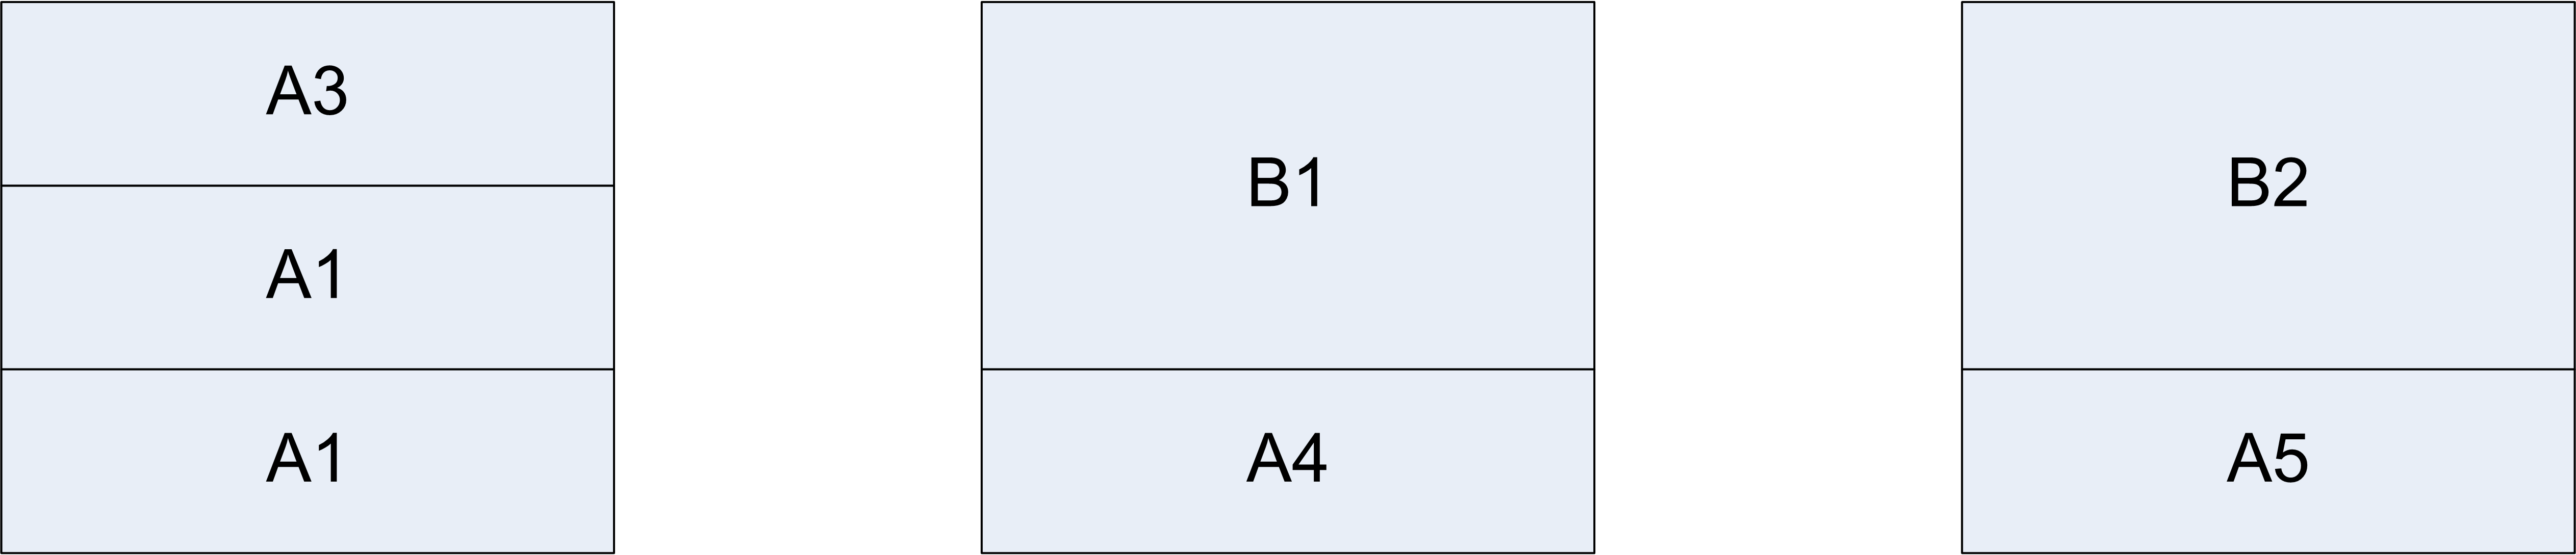
\includegraphics[width=5.5in]{images/ducc-internals/rm-structure-1.png}
      \caption{Unfragmented Layout}
      \label{fig:rm-fragmentation-1}
    \end{figure}

  However, as time proceeds and jobs come and go, it is possible that job A would get
  allocated as in Figure ~\ref{fig:rm-fragmentation-2}.  Now job B can only get 1 process: exactly HALF it's
  ``deserved'' allocation.  It would be necessary to preempt one of job A's processes to make space,
  even though job A is not above its fair-share allocation.

    \begin{figure}[H]
      \centering
      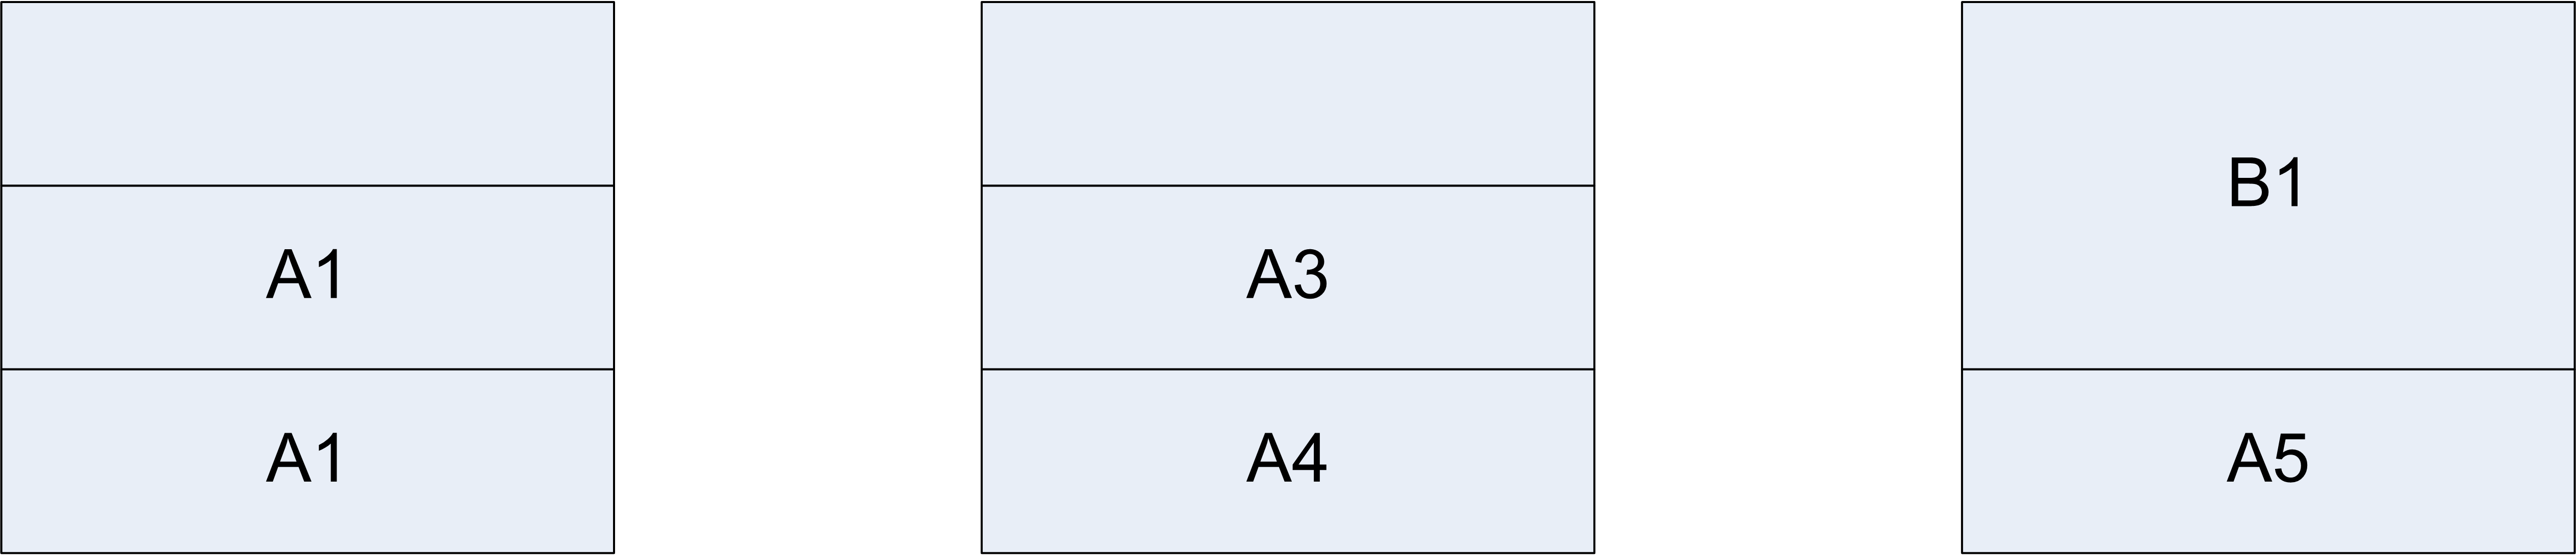
\includegraphics[width=5.5in]{images/ducc-internals/rm-structure-2.png}
      \caption{Fragmented Layout}
      \label{fig:rm-fragmentation-2}
    \end{figure}

  Of course this is a simplistic example.  In general the situation is significantly more complex.

  The goal of {\em defragmentation} is to reconfigure job A as in Figure ~\ref{fig:rm-fragmentation-1} so that
  job B can get its full allocation.

  The general procedure for defragmentation is as follows:

  \paragraph{Detection} This is performed in the method {\em detectFragmentation()}.
  After ``What Of'', all jobs are iterated.  Two numbers  are derived for each job:
  \begin{enumerate}
    \item The number of ``deserved'' shares.  During the ``How Much'' phase, 
      we perform a weighted fair-share assignment of resources. Often a job
      cannot use its full ``fair share'' allotment; for example, it may be a 
      new job and only need two initial processes.  The extra resources are
      apportioned to other jobs which end up with MORE than their proper
      weighted fair-share allotment.

      The ``deserved'' shares is a user's TRUE fair-share allotment, 
      calculated BEFORE bonus shares are allocated to it.  This number is
      calculated during the ``How Much'' phase and stored in each RmJob as
      the {\em pure\_fair\_share}.

    \item The number of allocated shares.  This number is calculated (in {\em RmJob}) as
\begin{verbatim}
   shares_allocated + pending_expansions - pending_preemptions
\end{verbatim}
    \end{enumerate}

    If the number of ``deserved'' shares is greater than the number of allocated
    shares (accounting for expansion and preemption), the job is considered
    ``potentially needy''.

    If there are no ``potentially needy'' jobs, {\em defragmentation} is done and
    we can proceed to broadcast the schedule.

    The second goal of defragmentation is to minimize ``churn'' in the system.  We
    do NOT attempt to achieve a perfect layout.  Instead, there is a threshold
    minimum number of processes we try to guarantee every job.  This number is configured
    in {\em ducc.properties} as the {\em ducc.rm.fragmentation.threshold}.

    A pass is now made over every ``potentially needy'' job.  Every such job with an
    allocation that is greater than the {\em fragmentation threshold} is removed from the
    ``needy'' list.  All remaining jobs are considered ``actually needy''.

    If there are no ``actually needy'' jobs, {\em defragmentation} is done and we can
    proceed to broadcast the schedule.

    Otherwise, the method {\em doFinalEvictions()} is called to try to make space for
    ``actually needy'' jobs.  We perform a ``take from the rich and give to the poor''
    procedure to insure that jobs whose allocation are below both their ``deserved fair share''
    and the ``fragmentation threshold'' are assigned additional resources.

    NOTE: This procedure works for non-preemptable allocations as well.  For non-preemptable
    allocations, the ``deserved'' value is exactly 1 {\em nshare} and any such job
    with no allocations is considered ``actually needy''.

    We iterate all users and add up the total {\em qshares} occupied by all their jobs,
    ordering the users by this value, known as their ``wealth''.

    We iterate the ``actually needy'' jobs.  For each such job we iterate the ``wealthy'' users,
    starting from the ``wealthiest'', inspecting their jobs to see if any of the processes are
    allocated over resources that can be allocated to the needy job.  Note that removal of a share
    must NOT result an an otherwise non-needy job becoming ``needy''.  If so, the user's wealth is
    decremented and one of two things occurs:
    \begin{enumerate}
      \item If the selected process is a ``pending expansion'' that has not been published,
        it is immediately reassigned to the needy job.  (Note that this is an optimization and
        the one exception to the rule that once a allocation is finalized in {\em RmJob}
        it cannot be changed.) If the job is no longer needy it
        is removed from the needy list.
      \item Otherwise, the selected process is preempted and the needy job is placed on
        a global ``needyJobs'' list.  Jobs on this list get priority allocation BEFORE
        any new allocations are made in all subsequent scheduling cycles, until they
        are no longer needy.
    \end{enumerate}
    
    Note the conditions which must be met by a process before it can be donated to a needy job
    (verified in method {\em takeFromTheRich()}):
    \begin{itemize}
      \item The machine containing the share must be of sufficient {\em share order}.
      \item The share must be preemptable.
      \item The machine must be in a compatible nodepool.
      \item If this share is evicted, the owning job must not become ``needy''.
      \item If this share is evicted, it must leave sufficient space on the machine for the new
        share.  i.e, if it is impossible to clear enough space on the machine for the needy job,
        there is no point evicting this share. We iterate all shares on the machine at this point
        and try to evict sufficient shares (which of course must belong to ``wealthy'' users) to
        make space for the needy share.
    \end{itemize}
             
\subsection{NodePool}

    The {\em NodePool} object manages physical nodes, represented in the RM by an
    object called {\em Machine}.  The collections of NodePools form a tree structure
    with each ``nested'' nodepool managed as a ``child'' of its ``parent'' nodepool.
    
    There are many more methods in NodePool than are documented here.  In this section
    we only review the most important, or the most complicated methods.

    The RM supports multiple disjoint NodePools, known as ``top-level'' nodepools.  The collection
    of ``top-level'' nodepools partitions the entire nodespace into independently scheduled
    resource collections.  The motivation is to permit multiple, disparate collections of nodes to
    be managed under a single DUCC system (rather than run multiple independent DUCC systems).

    Most of the NodePool algorithms are recursive.  Both the {\em Scheduler} and
    {\em NodePoolScheduler} object generally interact with the top NodePool of each
    tree, which coordinates, through recursion, the direction of requests to the 
    correct, possibly nested target NodePool.

    For example, to count the machines in a nodepool, one generally wants the count of
    machines in the pool PLUS the machines in its children:
\begin{verbatim}
    /**
     * How many do I have, including recusring down the children?
     */
    int countMachines()
    {
        int count = allMachines.size();
        for ( NodePool np : children.values() ) {
            count += np.countMachines();
        }
        return count;
    }
\end{verbatim}

    In the cases where recursion is to be inhibited, most of the methods are modified
    with the name ``Local'':
\begin{verbatim}
    /**
     * Non-recursive machine count.
     */
    int countLocalMachines()
    {
        return allMachines.size();
    }
\end{verbatim}

    Most of the methods in {\em NodePool} are short and easily understood, like the two above. There
    are a few subtleties in NodePool which will be expanded upon below.

\subsubsection{NodePool Reset}
    All scheduling phases must be aware of what physical resources are available, which are in use, and
    which are available for scheduling.  As we proceed with scheduling we need to maintain scratch-space
    that represents the current ``potential'' schedule, but without perturbing the existing allocations.
    
    The NodePool provides exactly this scratch space.  Before the two main scheduling phases, ``How
    Much'' and ``What Of'', the NodePool is instructed to reset().  The NodePool (and recursively,
    the entire set of nested NodePools), drops all of its structures other than the most basic Machine
    structures and then rebuilds them from the machine structures..  The scheduling phases then create
    ``trial'' schedules, resetting the NodePool as often as necessary.

    This also has the side-effect that errors do not tend to accumulate in the system; we essentially
    reboot the schedule on every pass.

    Finalizing the schedule is done in the Machine objects, with some help from the RmJob and
    Share objects.  

    (NOTE: as an optimization, RM does NOT generally rebuild Machine and RmJob from scratch on each
    Orchestrator publication.  They ARE rebuilt whenever RM starts, and during dynamic RM Reconfiguration).

    The next section, {\em Virtual Machines} provides a concrete example of the use of NodePool for
    scratch space during scheduling.

\subsubsection{Virtual Machines}
    Probably the most important part of the scheduler is encapsulated in the NodePool method,
    {\em rearrangeVirtual}.  This method treats the collection of all ``real'' machines as
    a collection of ``virtual'' machines which is the resource set that is scheduled against.

    In the RM's view, a ``virtual machine'' is any PROPER subset of a ``real machine''.  (Recall
    the mathematical definition of a PROPER subset is any subset of some set that is not equal
    to that set.). 

    As soon as an allocation of a single {\em nshare} is made against a machine, that machine's
    capacity for further allocations is diminished until the allocation is released by the Orchestrator.  For example, an
    order-3 allocation against an ``real'' order-5 machine results in the diminution of the order-5 machine
    to a ``virtual'' order-2 machine.  To put it differently, making a 3-quantum allocation against a 5-quantum
    ``real machine'' results in a 2-quantum ``virtual machine''.
    

    To understand what {\em rearrangeVirtual()} does it is important to understand three tables.
    These three tables are indexed by {\em share order} and are the key structures for both ``How
    Much'' and ``What Of''.  These tables are:
    \begin{description}
      \item[nMachinesByOrder] This table contains the number of full, free ``real machines'' with no allocations,
        indexed by {\em share order} 1, 2, ... {\em maxorder}.
      \item[vMachinesByOrder] This table contains the number of ``virtual machines'' indexed by {\em share order.}
      \item[nSharesByOrder]  This table contains the number of {\em nshares} of every order which can be
        currently allocated.
    \end{description}
    
    There is no overlap between ``nMachinesByOrder'' and ``vMachinesByOrder''. Therefore, the number
    of schedulable ``machines'' of any kind for some specific order {\em O} is
\begin{verbatim}
    nMachinesByOrder[O] + vMachinesByOrder[O]
\end{verbatim}

\paragraph{nSharesByOrder} is derived from the two machine tables and the meaning of its values
    is subtly different.  The numbers in the machine tables are independent of each other.  For example, if
    there is a single order-5 ``real machine'', this does NOT imply that there is also an order-3
    ``virtual machine'' and an order-2 ``virtual machine''.  This breakdown can only happen after
    allocation.

    {\em nSharesByOrder} however, gives the number of {\em nshares} of an order that might be
    allocated from any possible machine, real or virtual, allowing that a larger share may need to
    be split.  Each value in the table is dependent on the values of higher order in the table.  For
    example, if there is 1 order-5 ``real machine'', nSharesByOrder will indicate there is 1
    order-5 share available, or 1 order-4 share, or 1 order-3 share, or 2 order-2 shares, or 5
    order-1 shares.  Here is an example of what these tables might look like at some point during scheduling:
\begin{verbatim}
    Order                     1  2 3  4
    -------------------  ----------------
    nMachinesByOrder[];  [ 0  2  0 1  4 ] - physical machines
    vMachinesByOrder[];  [ 0  1  2 0  0 ] - virtual machines
    nSharesByOrder[]  ;  [ 0 26 11 5  4 ] - collective N Shares for each order
\end{verbatim}
    
\subsubsection{rearrangeVirtual(Machine M, order O)}
    We can now explain this method.  This is called when we wish to allocate a single
    {\em nshare} of order {\em O} from machine {\em M}.  The accounting works as follows:
    if the machine has no allocations, decrement {\em nMachinesByOrder[O]} by one; else
    decrement {\em vMachinesByOrder[O]} by one.  If the allocation would cause the 
    free space to be split, calculate the order of the free space after allocation and 
    increment the correct value in {\em vMachinesByOrder} like this:

    \paragraph{First Step}: Update the two machine tables.
\begin{verbatim}
    int v_order = M.getVirtualShareOrder();    // How much free space in the machine?
    int r_order = M.getShareOrder();           // How much total space in the machine?

    if ( v_order == r_order ) {                // Free == total?
        nMachinesByOrder[r_order]--;           // Yes, full machine allocation
    } else {
        vMachinesByOrder[v_order]--;           // No, virt machine allocation
    }

    v_order -= O;                              // Does it cause a split?
    if ( v_order > 0 ) {                       // Yes
        vMachinesByOrder[v_order]++;           // Add a "new", smaller virt machine
    }
\end{verbatim}
    There are, of course, additional details, which can be seen by inspecting the
    full source listing.

    \paragraph{Second Step} Update the share table.  We initialize the table with the total of real
    and virtual machines by order.  Then in a double iteration, look ``forward'' to count the number
    of shares that might be acquired from higher order allocations by splitting the space.  The full
    method is included here for the curious.  Everyone else can simply trust that it is correct.
\begin{verbatim}
    protected void calcNSharesByOrder()
    {
        int len = nMachinesByOrder.length;

        // init nSharesByorder to the sum of 'n and 'v MachinesByOrder
        System.arraycopy(nMachinesByOrder, 0, nSharesByOrder, 0, len);
        for ( int i = 0; i < getMaxOrder() + 1; i++ ) {
            nSharesByOrder[i] += vMachinesByOrder[i];
        }

        for ( int o = 1; o < len; o++ ) {                     // counting by share order
            for ( int p = o+1; p < len; p++ ) {
                if ( nSharesByOrder[p] != 0 ) {
                    nSharesByOrder[o] += (p / o) * nSharesByOrder[p];
                }
            }
        }
    }
\end{verbatim}
    
\subsubsection{connectShare(Share s, Machine m, IRmJob j, int order)}
    This helper method is responsible for updating all the records in order to
    allocate a specific share on a specific machine for a specific job.  Its
    action is irreversible: once this method is called, the share is irrevocably
    assigned to the given job on the given machine (except sometimes, during
    defragmentation, as described above).

    {\em rearrangeVirtual()} is called at the end to update the internal ``counts''.

\subsubsection{compatibleNodepool(Policy p,  ResourceClass rc)}
    This method determines if the current nodepool is compatible with the indicated
    scheduling policy and resource class.  If the policy is FAIR\_SHARE, recursion
    through the child nodes is performed.

\subsubsection{nodeArrives}
    This straightforward method adds a node to the list of schedulable nodes.  It updates the
    database, deals with unresponsive nodes becoming responsive again, and does
    simple bookeeping.

\section{RmJob}

    The RmJob is mostly an accounting object.  While its implementation has many details,
    there are two important methods: {\em calcJobCaps()} and {\em shrinkBy(int count)}, both
    of which were briefly mentioned above.

\subsection{calcJobCaps()}
    If the {\em rearrangeVirtual()} code described above has a rival for ``most important method'',
    it would be the RmJob's {\em calcJobCaps()}.  This method is called many times throughout
    scheduling and is required to return {\em exactly} the number of shares the job could make
    use of at the current moment, if there were unbounded resources.

    Note that this is the method to modify if you wish to change the rate of expansion or
    contraction of a job.

    Because it is called so often, the scheduler iterates all jobs at the start of each 
    scheduling cycle and calls {\em initJobCap()} to calculate the cap based on current job
    state.  This caches the actual cap, which is returned in subsequent calls to
    {\em calcJobCaps()}.

    The design point is this:  Estimate the cap as the largest value that is meaningful.  Then
    whittle it down to the minimum by applying the architected constraints such as
    the ``initialization cap'' and prediction of when we expect the job to complete.  We want
    everything we can get but no more than we can use.

    This code can be tricky to understand so we'll present it here.  The returned ``actual\_cap'' is
    the value used by NodePoolScheduler's ``How Much'' phase for all {\em entities} to determine share allocations.

    The following steps are taken by {\em initJobCap()}:
    \begin{enumerate}
      \item If the job is unschedulable (refused), set cap to 0 and return. (No shares will be allocated.)
      \item If the job is completed but not yet deallocated, set the cap to the total shares
        it already has allocated and return. (No additional shares will be allocated.)
        \item Set the tentative cap to the number of remaining {\em work items}  divided by the declared
          threads per processes.  This is the upper bound on the cap:
\begin{verbatim}
     c = (n_remaining_questions / nthreads}
\end{verbatim}

        \item Adjust the tentative cap to the maximum of ``c'' and the number of shares already
          allocated.  This accounts for jobs ``winding down'' when work items start to vacate
          processes so we have more processes than are needed for the remaining work but we 
          want to insure that ``How Much'' does not cause premature shrinkage.
\begin{verbatim}
        int currentResources = countNShares();
        c = Math.max(c, currentResources); 
\end{verbatim}

        \item Adjust the tentative cap to the minimum of ``c'' and the declared {\em process\_deployments\_max}.
          Call this the ``base cap''.  It is the job cap before accounting for prediction and is
          used if we cannot find a better estimate.
\begin{verbatim}
        int base_cap = Math.min(getMaxShares(), c);
\end{verbatim}
          
        \item Predict the number of shares this job could use on an unbounded system,
          based on the average initialization time of its processes and the rate of completion
          of the work items so far.  Call this the ``projected\_cap''.
\begin{verbatim}
        int projected_cap = getProjectedCap();      
        if ( projected_cap == 0 ) {                   // we know nothing, this is best guess
        	projected_cap = base_cap;
        }
\end{verbatim}

        \item All else being equal, the potential cap for the job is now the max of the actual
          resources we have allocated, and the projected cap.  It is the largest number of
          resources we believe the job can ever use.
\begin{verbatim}
        potential_cap = Math.max(projected_cap, currentResources);
\end{verbatim}

            \item If we're still initializing, and we have configured {\em ducc.rm.initialization.cap}
              in {\em ducc.properties}, revise the cap down and return the {\em actual\_cap}.
\begin{verbatim}
        actual_cap = Math.min(potential_cap, (resource_class.getInitializationCap()));
\end{verbatim}

            \item If we're still initializing and we do NOT have an initiation cap configured,
              set the {\em actual\_cap} to the {\em potential\_cap} and return.
\begin{verbatim}
        actual_cap = potential_cap
\end{verbatim}
              
            \item If we've completed at least one initialization, and we have configured
              {\em ducc.rm.expand.by.doubling}, return the smaller of the {\em potential\_cap}
              and TWICE the currently allocated resources:
\begin{verbatim}
       actual_cap = Math.min(potential_cap, currentResources * 2);
\end{verbatim}

            \item If we've completed at least one initialization, and we do NOT use
              expand-by-doubling, return the {\em potential\_cap}
\begin{verbatim}
       actual_cap = potential_cap
\end{verbatim}

              \item There is one last corner case.  It is possible the job has
                shrunk to 0 resources (pushed out by fair-share for example). If
                this has happened we have to restart the doubling, and we need to
                ask for at least the initialization cap.  But we don't want to go
                over the ``base\_cap'' which has accounted for the fact the job might
                be running down and we can't use the full initialization cap.
\begin{verbatim}
      if ( currentResources == 0 ) {
         actual_cap = Math.max(1, resource_class.getInitializationCap()); 
         actual_cap = Math.min(base_cap, actual_cap);                     
       }
\end{verbatim}


        \end{enumerate}
    
\subsection{shrinkBy(int count)}
    This is a rather trivial method, used to implement ``shrink by investment''.  Originally
    this was a much more involved processes, which gradually became refined to its current
    incarnation.

    All this method does is sort the RmJob shares as described in the interlude above, ``Preemptions'',
    and deletes the indicated number of shares from the front of the sorted list.

    The original {\em shrinkByInvestment()} code has been left in place for reference.

\section{Supporting Classes}
   There are a number of supporting classes mostly used for bookkeeping, mentioned here for completeness.

\subsection{Machine}
This represents a Node.  A Machine object is created whenever a Node's state arrives.  The Machine
is entered into an appropriate nodepool.  Machine objects are NEVER destroyed (except during dynamic
reconfiguration) as it is usually expected that an unresponsive machine will become responsive
again.  This significantly reduces the complexity of bookkeeping.

\subsubsection{Blacklists and Whitelists}
The Machine maintains a list of {\em Share}s allocated to it.  It is possible, after changing the
{\em ducc.classes} configuration and starting RM, that it is no longer legal for these shares to be
allocated on this machine, or perhaps to be allocated at all.  For example the machine may have been
moved to a different class than the class of the work allocated on it, or the class may be been
deleted entirely.

   If this happens the shares are essentially in ``limbo''.  They cannot (in general) be associated
   with any resource class and therefore cannot participate in allocations (recall, allocations are
   done by resource class).  The space must nonetheless be accounted for to avoid double-booking the nodes.

   To cope with this the RM considers both the {\em Shares}, and the {\em Machine} they reside on
   to be ``blacklisted''.  When a machine is ``blacklisted'',
   \begin{itemize}
     \item All work that can be evicted from it is evicted.  This include any kind of UIMA-AS
       job (including jobs submitted to non-preemptable classes),  and Services.
     \item No additional allocations can be made to the machine until ALL blacklisted work
       has been confirmed by the Orchestrator to have left the system.
   \end{itemize}
   
    Once all blacklisted work on a machine has left the system, the machine is ``white-listed'' and
    allocations on it are resumed.

\subsubsection{Database and Persistence}
   When any machine arrives in the system, a new record is entered in the database containing its
   essential data.

   All state subsequent changes for the machine are entered into the database, including the number
   of missed consecutive Agent heartbeats.

   When a share is assigned to a machine, or leaves a machine, it is the responsibility of the Machine object to
   record the share and its details in the database.

\subsection{Share}
    The Share object represents one full allocation.  Internally it is an {\em nshare} and thus
    has share order, where the {\em share order} is the number of {\em qshares} it represents.  A
    share is logically exposed outside of RM as a Process.

    The Share's main purpose is bookkeeping; a place to store investment, initialization time and
    to represent the space occupied by a resource allocation.

\subsection{ResourceClass}

    The ResourceClass represents the {\em class} concept as configured in {\em ducc.classes}.  It
    holds the configured class rules (expand\_by\_doubling, initialization\_cap, etc).

    It's primary purpose is bookkeeping; a place to organize jobs by class, jobs by user by class,
    to maintain the set of users authorized for the class, etc.  It also tracks non-preemptable
    share {\em allotment}.

    The {\em ResourceClass} is a schedulable {\em IEntity}, as described above in the description
    of the FAIR\_SHARE algorithm.

\subsection{User}

    The User represents a single user. Its primary purpose is bookkeeping; a place to organize
    jobs owned by the user.

    The User is a schedulable {\em IEntity}, as described above in the description of the 
    FAIR\_SHARE algorithm.

\subsection{JobManagerUpdate}

    This is a ``transfer object'' used to transfer the current schedule to the publication
    mechanism and ultimately to the Orchesrator.  It consist of maps of all shares, organized
    by shares ``expanded'', and ``shrunken'' (preempted).  The RM's publication mechanism
    translates this into the appropriate format which then gets published to the Orchestrator.
    
